
\documentclass[10pt]{beamer}


\mode<presentation>
{
 \usetheme{Boadilla}
\pagestyle{empty}

\setbeamerfont*{frametitle}{size=\normalsize,series=\bfseries}
\setbeamerfont*{block}{size=\normalsize,series=\bfseries}
%\setbeamertemplate{blocks}[rounded][shadow=true]
}

\usepackage{epsfig,epstopdf}
\usepackage{etex}
% \usepackage{helvet}
\usepackage{amsmath, amssymb}
\usepackage{color}
\usepackage{asymptote}
\usepackage{mathrsfs}
\usepackage{dsfont}
\usepackage{makeidx}
\usepackage{multido}
\usepackage{adjustbox}
\usepackage{cancel}

\usepackage{pst-sigsys,pst-plot,pstricks-add}
\usepackage{pst-pdf}

\usepackage[american voltages, american currents,siunitx]{circuitikz}
%\sisetup{load=derived} % loading \siemens


\makeatletter
% create the shape
\pgfcircdeclarebipole{}{\ctikzvalof{bipoles/interr/height 2}}{spst}{\ctikzvalof{bipoles/interr/height}}{\ctikzvalof{bipoles/interr/width}}{

    \pgfsetlinewidth{\pgfkeysvalueof{/tikz/circuitikz/bipoles/thickness}\pgfstartlinewidth}

    \pgfpathmoveto{\pgfpoint{\pgf@circ@res@left}{0pt}}
    \pgfpathlineto{\pgfpoint{.6\pgf@circ@res@right}{\pgf@circ@res@up}}
    \pgfusepath{draw}   
}

% make the shape accessible with nice syntax
\def\pgf@circ@spst@path#1{\pgf@circ@bipole@path{spst}{#1}}
\tikzset{switch/.style = {\circuitikzbasekey, /tikz/to path=\pgf@circ@spst@path, l=#1}}
\tikzset{spst/.style = {switch = #1}}
\makeatother





\definecolor{links}{HTML}{2A1B81}
\hypersetup{colorlinks,linkcolor=,urlcolor=links}

\def\nn{\nonumber}

\definecolor{links}{HTML}{2A1B81}
\hypersetup{colorlinks,linkcolor=,urlcolor=links}


\title[]{RC and RL circuits}
\author[\textcolor{blue}{Systems and Circuits}]{\textcolor{darkblue}{Pablo M. Olmos} (olmos@tsc.uc3m.es)\\ \textcolor{darkblue}{Emilio Parrado} (emipar@tsc.uc3m.es)}
\institute{\textcolor{white}{UC3M}}

\definecolor{darkblue}{rgb}{0.0, 0.0, 0.40}
\setbeamercolor{title}{fg=darkblue}
\setbeamercolor{frametitle}{fg=darkblue}
\definecolor{darkgreen}{rgb}{0.0, 0.4, 0.0}



\AtBeginSection[]
{
  \begin{frame}<beamer>{Index}
    \tableofcontents[currentsection,currentsubsection]
  \end{frame}
}

\begin{document}
\frame{
\titlepage
\thispagestyle{empty}
\begin{center}
\includegraphics[scale=0.05]{Figures/uc3m-logo.pdf}
\end{center}
}

\section{Quick review: capacitors and inductors}


\frame{
\frametitle{The Capacitor}
\begin{block}{}
\begin{columns}
\begin{column}{0.2\textwidth}
\begin{center}
\begin{circuitikz} \draw[black]
(0,0) to[C=$C$,i>=$i(t)$,v=$v(t)$] (2,0);
\end{circuitikz}
\end{center}\end{column}
\begin{column}{0.2\textwidth}
\begin{align}\nn
i(t)&=C\frac{d v(t)}{d t}
\end{align}
\end{column}
\begin{column}{0.5\textwidth}
\begin{align}\nn
v(t)&=\frac{1}{C}\int_{t_0}^{t}i(\tau)\text{d}\tau+v(t_0)
\end{align}
\end{column}
\end{columns}
\end{block}

From the definition of power
\begin{align*}
p(t)=v(t)i(t)=Cv(t)\frac{dv(t)}{dt}
\end{align*}
or
\begin{align*}
p(t)=v(t)i(t)=i(t)\left[\frac{1}{C}\int_{t_0}^{t}i(\tau)\text{d}\tau+v(t_0)\right]
\end{align*}

The energy in the capacitor at any time can be computed as follows:
\begin{align*}
p(t)=\frac{d w(t)}{d(t)}\Rightarrow w(t)=\int_{-\infty}^{t} p(\tau) d\tau=\int_{-\infty}^{\tau}  v(\tau) C\frac{d v(\tau)}{\cancel{d \tau}} \cancel{d\tau}=C\frac{v^2(t)}{2}
\end{align*}

}

\frame{
\frametitle{Capacitors in parallel/series}

\begin{circuitikz} \draw[black]
(-2,0) to[short,o-] (5,0)
(-2,2) to[short,o-] (5,2)
(0,0) to[C=$C_1$] (0,2)
(2,0) to[C=$C_2$] (2,2)
(5,0) to[C=$C_N$] (5,2)
(3,1) node[]{\ldots}
(7,0)to[C,o-o](7,2)
(9,1) node[]{$C_{eq}=\sum_{i}C_i$};
\end{circuitikz}
\vspace{1.5cm}

\begin{circuitikz} \draw[black]
(0,0) to[C=$C_1$,o-] (1.5,0)
to[C=$C_2$] (3,0)
(4,0) node[]{$\ldots$}
(5,0) to[C=$C_N$,-o] (6.5,0)
(8,0)to[C,o-o](10,0)
(9,1) node[]{$C_{eq}=\left(\sum_{i}\frac{1}{C_i}\right)^{-1}$};
\end{circuitikz}



}

\frame{
\frametitle{The Inductor}
\begin{block}{}
\begin{columns}
\begin{column}{0.2\textwidth}
\begin{center}
\begin{circuitikz} \draw[black]
(0,0) to[L=$L$,i>=$i$,v=$v$] (2,0);
\end{circuitikz}
\end{center}\end{column}
\begin{column}{0.2\textwidth}
\begin{align}\nn
v(t)&=L\frac{d i(t)}{d t}
\end{align}
\end{column}
\begin{column}{0.5\textwidth}
\begin{align}\nn
i(t)&=\frac{1}{L}\int_{t_0}^{t}v(\tau)\text{d}\tau+i(t_0)
\end{align}
\end{column}
\end{columns}
\end{block}

From the definition of power
\begin{align*}
p(t)=v(t)i(t)=Li(t)\frac{di(t)}{dt}
\end{align*}
or
\begin{align*}
p(t)=v(t)i(t)=v(t)\left[\frac{1}{L}\int_{t_0}^{t}v(\tau)\text{d}\tau+i(t_0)\right]
\end{align*}

The energy in the inductor at any time can be computed as follows:
\begin{align*}
p(t)=\frac{d w(t)}{d(t)}\Rightarrow w(t)=\int_{-\infty}^{t} p(\tau) d\tau=\int_{-\infty}^{t}  i(\tau) L\frac{i v(\tau)}{\cancel{d \tau}} \cancel{d\tau}=L\frac{i^2(t)}{2}
\end{align*}

}




\frame{
\frametitle{Inductors in parallel/series}

\begin{circuitikz} \draw[black]
(-2,0) to[short,o-] (5,0)
(-2,2) to[short,o-] (5,2)
(0,0) to[L=$L_1$] (0,2)
(2,0) to[L=$L_2$] (2,2)
(5,0) to[L=$L_N$] (5,2)
(3,1) node[]{\ldots}
(7,0)to[L,o-o](7,2)
(9,1) node[]{$L_{eq}=\left(\sum_{i}\frac{1}{L_i}\right)^{-1}$};
\end{circuitikz}
\vspace{1.5cm}

\begin{circuitikz} \draw[black]
(0,0) to[L=$L_1$,o-] (1.5,0)
to[L=$L_2$] (3,0)
(4,0) node[]{$\ldots$}
(5,0) to[L=$L_N$,-o] (6.5,0)
(8,0)to[L,o-o](10,0)
(9,1) node[]{$L_{eq}=\sum_{i}L_i$};
\end{circuitikz}



}


\section{General solution of the first order linear differential equation}

\frame{
\frametitle{First order linear differential equation with constant coefficients}
Compute $y(t)$ such that $y(t_0)=y_0$ if 
%\begin{align}\nn
%A\frac{dx(t)}{dt}+Bx(t)=C
%\end{align}
%where $A$, $B$ and $C$ are constants.
%
%\begin{align}\nn
%\alpha\frac{dx(t)}{dt}+\beta x(t)=\gamma
%\end{align}
%where $\alpha$, $\beta$ and $\gamma$ are constants.
%
\begin{align}\nn
\frac{dy(t)}{dt}+\frac{1}{\tau}y(t)=\gamma
\end{align}
where $\tau$ and $\gamma$ are constants.

\begin{exampleblock}{Sol.}
\begin{align}\nn
y(t)=\tau\gamma\left(1-\text{e}^{-\frac{(t-t_0)}{\tau}}\right)+y_0\text{e}^{-\frac{(t-t_0)}{\tau}}\qquad t\geq t_0
\end{align}
\end{exampleblock}
}

\section{RC circuits}


\frame{
\begin{itemize}
\item We now determine the currents and voltages that arise in simple circuits when the energy stored in either an inductor or a capacitor is released or acquired.
\item We first focus on the RC circuit: a single capacitor, a resistor and a source.
\end{itemize}



\begin{center}
\begin{circuitikz}[] \draw[black]
(-2,0) to[V=$V_s$] (-2,2)
(-2,2) to[R=$R_s$] (0,2)
to[switch] (2,2)
to[C=$C$,v=$V_C$] (2,0)
(2,2) to[switch] (4,2)
to[R=$R$] (4,0)
to[short] (-2,0);
%(6,0) to[V=$V_s$] (6,2)
%to[switch] (8,2)
%to[C=$C$] (8,0)
%(8,2) to[short] (10,2)
%to[R=$R$] (10,0)
%to[short] (6,0)
%%(2,3) node[] {$t<t_0$}
%%(8,3) node[] {$t\geq t_0$}
%(6,0) node[ground] {}
%(8,2.25) node[] {A};
\end{circuitikz}
\end{center}

}

%
%\frame{
%We divide our analysis in two phases:
%\begin{enumerate}
%\item We consider the currents and voltages that arise when stored energy in a capacitor is suddenly released to a resistive network. This is called the \textbf{natural response} of the circuit.
%\item Then we discuss the problem of finding currents and voltages generated in RC circuits when either constant voltage and current sources are applied to the circuit. This is called the \textbf{natural response} of the circuit.
%\end{enumerate}
%
%\begin{center}
%\begin{tabular}{cc}
%\begin{circuitikz} \draw[black]
%(2,2) to[C,v=$V_C$] (2,0)
%(2,2) to[cspst=$t_0$] (4,2)
%to[R=$R$] (4,0)
%to[short] (2,0);
%\end{circuitikz}&
%\begin{circuitikz}[] \draw[black]
%(-2,0) to[V=$V_s$] (-2,2)
%(-2,2) to[R=$R_s$] (0,2)
%to[cspst=$t_0$] (2,2)
%to[C=$C$,v=$V_C$] (2,0)
%(2,2) to[short] (4,2)
%to[R=$R$] (4,0)
%to[short] (-2,0);
%\end{circuitikz}\\\\
%$V_C(t_0^{-})=V_0$ & $V_C(t_0^{-})=0$\\\\
%\textbf{Natural response} & \textbf{Step response}
%\end{tabular}
%\end{center}
%
%
%}


\frame{
\frametitle{Natural response of the RC circuit}

 
\begin{center}
\begin{circuitikz} \draw[black]
(2,2) to[C,v=$V_C$,i>=$i$] (2,0)
(2,2) to[cspst=$t_0$] (4,2)
to[R=$R$] (4,0)
to[short] (2,0)
(3,3) node[] {$V_C(t_0^{-})=V_0$};
\end{circuitikz}
\end{center}


\textbf{Kirchhoff's voltage law ($t\geq0$):}
\begin{align}\nn
V_C(t)+iR=0\Rightarrow V_C(t)+RC\frac{dV_C(t)}{dt}=0
\end{align}
}

\frame{
\frametitle{}

\begin{exampleblock}{}
\begin{columns}
\begin{column}{0.2\textwidth}
\begin{align}\nn
\frac{dy(t)}{dt}+\frac{1}{\tau}y(t)=\gamma
\end{align}
\end{column}
\begin{column}{0.2\textwidth}
\begin{align}\nn
y(t_0)=y_0
\end{align}
\end{column}
\begin{column}{0.5\textwidth}
\begin{align}\nn
y(t)=\tau\gamma\left(1-\text{e}^{-\frac{(t-t_0)}{\tau}}\right)+y_0\text{e}^{-\frac{(t-t_0)}{\tau}}
\end{align}
\end{column}
\end{columns}
\end{exampleblock}

If $V_C(t_0^{-})=V_0$ and 
\begin{align}\nn
V_C(t)+RC\frac{dV_C(t)}{dt}=0
\end{align}
then $\tau=RC$ and $\gamma=0$.
\begin{block}{}
\begin{align}\nn
V_C(t)=V_0\text{e}^{-\frac{(t-t_0)}{RC}}\qquad t\geq t_0
\end{align}
\end{block}
}


\frame{
\frametitle{Natural response of the RC circuit}
\begin{center}
\begin{circuitikz} \draw[black]
(2,2) to[C,v=$V_C$,i>=$i$] (2,0)
(2,2) to[cspst=$t_0$] (4,2)
to[R=$R$] (4,0)
to[short] (2,0)
(3,3) node[] {$V_C(t)=V_0\text{e}^{-\frac{(t-t_0)}{RC}}\qquad t\geq t_0$};
\end{circuitikz}
\end{center}
The current $i(t)$ is 
\begin{align}\nn
i(t)=C\frac{dV_C(t)}{dt}=-\frac{V_0}{R}\text{e}^{-\frac{(t-t_0)}{RC}}\qquad t\geq t_0
\end{align}
\begin{block}{}
The power in the capacitor $p(t)=i(t)V_C(t)<0$. What does it mean?
\end{block}
\begin{alertblock}{}
How is the natural response of the circuit if $V_0=0$?
\end{alertblock}

}

\frame{
\frametitle{Step response of the RC circuit}

\begin{center}
\begin{circuitikz}[] \draw[black]
(-2,0) to[V=$V_s$] (-2,2)
(-2,2) to[R=$R_s$,i>=$i_s$] (0,2)
to[cspst=$t_0$] (2,2)
to[C=$C$,v=$V_C$,i>=$i$] (2,0)
(2,2) to[short] (4,2)
to[R=$R$,i>=$i_R$] (4,0)
to[short] (-2,0)
(2,3) node[] {$V_C(t_0^{-})=0$}
(2,0) node[ground]{};
\end{circuitikz}
\end{center}

\begin{align}\nn
&i_s=i+i_R\Rightarrow \frac{(V_s-V_C(t))}{R_s}=C\frac{dV_C(t)}{dt}+\frac{V_C(t)}{R}\\\nn
&V_C(t)(R_s^{-1}+R^{-1})+C\frac{dV_C(t)}{dt}=\frac{V_s}{R_s}
\end{align}

}

\frame{
\frametitle{}


\begin{exampleblock}{}
\begin{columns}
\begin{column}{0.2\textwidth}
\begin{align}\nn
\frac{dy(t)}{dt}+\frac{1}{\tau}y(t)=\gamma
\end{align}
\end{column}
\begin{column}{0.2\textwidth}
\begin{align}\nn
y(t_0)=y_0
\end{align}
\end{column}
\begin{column}{0.5\textwidth}
\begin{align}\nn
y(t)=\tau\gamma\left(1-\text{e}^{-\frac{(t-t_0)}{\tau}}\right)+y_0\text{e}^{-\frac{(t-t_0)}{\tau}}
\end{align}
\end{column}
\end{columns}
\end{exampleblock}

If $V_C(t_0^{-})=0$ and 
\begin{align}\nn
V_C(t)(R_s^{-1}+R^{-1})+C\frac{dV_C(t)}{dt}=\frac{V_s}{R_s}
\end{align}
then $\tau=CR_{eq}$, where  $R_{eq}=(R_s^{-1}+R^{-1})^{-1}$ and $\gamma=\frac{V_s}{C R_s}$.
\begin{block}{}
\begin{align*}
V_C(t)=V_s\frac{R}{R_s+R}\left(1-\text{e}^{-\frac{(t-t_0)}{R_{eq}C}}\right), \qquad t\geq t_0.
\end{align*}
\end{block}
}

\frame{
\frametitle{Stationary regime}

In the limit $t\rightarrow\infty$, all currents and voltages are constant and the capacitor behaves like an open circuit. We can easily compute $\lim_{t_\rightarrow \infty}V_C(t)\doteq V_C^{\infty}$:

\begin{columns}
\begin{column}{0.6\textwidth}
\begin{center}
\begin{circuitikz}[] \draw[black]
(-2,0) to[V=$V_s$] (-2,2)
(-2,2) to[R=$R_s$,i>=$i_s$] (0,2)
to[short] (2,2)
to[short] (2,1.5)
(2,0) to[short] (2,0.5)
(1.5,1.5) to[open,v=$V^{\infty}_C$] (1.5,0.5)
(2,2) to[short] (4,2)
to[R=$R$,i>=$i_R$] (4,0)
to[short] (-2,0)
(2,0) node[ground]{};
\end{circuitikz}
\end{center}
\end{column}
\begin{column}{0.4\textwidth}
\begin{align}\nn
V_C^{\infty}=V_s\frac{R}{R_s+R}
\end{align}
\end{column}
\end{columns}

\vspace{0.5cm}
Which, obviously, coincides with
\begin{align*}
\lim_{t\rightarrow\infty}  V_s\frac{R}{R_s+R}\left(1-\text{e}^{-\frac{(t-t_0)}{R_{eq}C}}\right)=V_s\frac{R}{R_s+R}
\end{align*}


}


\frame{

\begin{center}
\begin{circuitikz}[] \draw[black]
(-2,0) to[V=$V_s$] (-2,2)
(-2,2) to[R=$R_s$,i>=$i_s$] (0,2)
to[cspst=$t_0$] (2,2)
to[C=$C$,v=$V_C$,i>=$i$] (2,0)
(2,2) to[short] (4,2)
to[R=$R$,i>=$i_R$] (4,0)
to[short] (-2,0)
(2,3) node[] {$V_C(t)=V_s\frac{R}{R_s+R}\left(1-\text{e}^{-\frac{(t-t_0)}{R_{eq}C}}\right), \qquad t\geq t_0$}
(2,0) node[ground]{};
\end{circuitikz}
\end{center}

\begin{block}{Current through the capacitor}
\begin{align}\nn
i(t)=C\frac{\partial V_C(t)}{\partial t}=V_s\frac{R}{R+R_s}\frac{1}{R_{eq}}\text{e}^{-\frac{(t-t_0)}{R_{eq}C}}=\frac{V_s}{R_s}\text{e}^{-\frac{(t-t_0)}{R_{eq}C}}
\end{align}
\end{block}

\begin{itemize}
\item Compute the power $p(t)$ in the capacitor over time. 
\item Homework: Compute the step response of the circuit if $V_C(t^{-}_0)=V_0$.
\end{itemize}

}


\section{RL circuits}


\frame{
\begin{itemize}
\item We now focus on the RL circuit: a single inductor, a resistor network and a source.
\end{itemize}



\begin{center}
\begin{circuitikz}[] \draw[black]
(-2,0) to[I=$I_s$] (-2,2)
to[short](-0.5,2)
(-0.5,0) to[R=$R_s$] (-0.5,2)
to[switch] (2,2)
to[L=$L$,i>=$i_L$] (2,0)
(2,2) to[switch] (4,2)
to[R=$R$] (4,0)
to[short] (-2,0);
%(6,0) to[V=$V_s$] (6,2)
%to[switch] (8,2)
%to[C=$C$] (8,0)
%(8,2) to[short] (10,2)
%to[R=$R$] (10,0)
%to[short] (6,0)
%%(2,3) node[] {$t<t_0$}
%%(8,3) node[] {$t\geq t_0$}
%(6,0) node[ground] {}
%(8,2.25) node[] {A};
\end{circuitikz}
\end{center}

}

%
%\frame{
%
%We divide our analysis in two phases:
%\begin{enumerate}
%\item We consider the currents and voltages that arise when stored energy in an inductor is suddenly released to a resistive network. This is called the \textbf{natural response} of the circuit.
%\item Then we discuss the problem of finding currents and voltages generated in RL circuits when either constant voltage and current sources are applied to the circuit. This is called the \textbf{natural response} of the circuit.
%\end{enumerate}
%
%
%
%\begin{center}
%\begin{tabular}{cc}
%\begin{circuitikz} \draw[black]
%(2,2) to[L=$L$,i>=$i_L$] (2,0)
%(2,2) to[cspst=$t_0$] (4,2)
%to[R=$R$] (4,0)
%to[short] (2,0);
%\end{circuitikz}&
%\begin{circuitikz}[] \draw[black]
%(-2,0) to[I=$I_s$] (-2,2)
%to[short](-0.5,2)
%(-0.5,0) to[R=$R_s$] (-0.5,2)
%to[cspst=$t_0$] (2,2)
%to[L=$L$,i>=$i_L$] (2,0)
%(2,2) to[short] (4,2)
%to[R=$R$] (4,0)
%to[short] (-2,0);
%\end{circuitikz}\\\\
%$i_L(t_0^{-})=I_0$ & $i_L(t_0^{-})=0$\\\\
%\textbf{Natural response} & \textbf{Step response}
%\end{tabular}
%\end{center}

%
%
%\begin{columns}
%\begin{column}{0.3\textwidth}
%\begin{center}
%\begin{center}
%\begin{circuitikz} \draw[black]
%(2,2) to[L=$L$,i>=$i_L$] (2,0)
%(2,2) to[cspst=$t_0$] (4,2)
%to[R=$R$] (4,0)
%to[short] (2,0)
%(3,3) node[] {$i_L(t_0^{-})=I_0$}
%(3,-1) node[]{\textbf{Natural response.}};
%\end{circuitikz}
%\end{center}
%\end{center}\end{column}
%\begin{column}{0.7\textwidth}
%\begin{center}
%\begin{circuitikz}[] \draw[black]
%(-2,0) to[I=$I_s$] (-2,2)
%to[short](-0.5,2)
%(-0.5,0) to[R=$R_s$] (-0.5,2)
%to[cspst=$t_0$] (2,2)
%to[L=$L$,i>=$i_L$] (2,0)
%(2,2) to[short] (4,2)
%to[R=$R$] (4,0)
%to[short] (-2,0)
%(1,3) node[] {$i_L(t_0^{-})=0$}
%(1,-1) node[]{\textbf{Step response.}};
%\end{circuitikz}
%\end{center}
%
%\end{column}
%\end{columns}



%}


\frame{
\frametitle{Natural response of the RL circuit}

\begin{center}
\begin{circuitikz} \draw[black]
(2,2) to[L=$L$,i>=$i_L$,v<=$V_L$] (2,0)
(2,2) to[cspst=$t_0$] (4,2)
to[R=$R$] (4,0)
to[short] (2,0)
(3,3) node[] {$i_L(t_0^{-})=I_0$}
(3,-1) node[]{\textbf{Natural response.}};
\end{circuitikz}
\end{center}

\textbf{Kirchhoff's voltage law ($t\geq t_0$):}
\begin{align}\nn
V_L(t)+i_L(t)R=0\Rightarrow i_L(t) R+L\frac{di_L(t)}{dt}=0
\end{align}
}


\frame{
\frametitle{}


\begin{exampleblock}{}
\begin{columns}
\begin{column}{0.2\textwidth}
\begin{align}\nn
\frac{dy(t)}{dt}+\frac{1}{\tau}y(t)=\gamma
\end{align}
\end{column}
\begin{column}{0.2\textwidth}
\begin{align}\nn
y(t_0)=y_0
\end{align}
\end{column}
\begin{column}{0.5\textwidth}
\begin{align}\nn
y(t)=\tau\gamma\left(1-\text{e}^{-\frac{(t-t_0)}{\tau}}\right)+y_0\text{e}^{-\frac{(t-t_0)}{\tau}}
\end{align}
\end{column}
\end{columns}
\end{exampleblock}

If $i_L(t_0^{-})=I_0$ and 
\begin{align}\nn
i_L(t) R+L\frac{di_L(t)}{dt}=0
\end{align}
then $\tau=L/R$ and $\gamma=0$.
\begin{block}{}
\begin{align*}
i_L(t)=I_0\text{e}^{-\frac{R}{L}(t-t_0)}\qquad t\geq t_0
\end{align*}
\end{block}
}


\frame{
\frametitle{Natural response of the RL circuit}

\begin{center}
\begin{circuitikz} \draw[black]
(2,2) to[L=$L$,i>=$i_L$,v<=$V_L$] (2,0)
(2,2) to[cspst=$t_0$] (4,2)
to[R=$R$] (4,0)
to[short] (2,0)
(3,3) node[] {$i_L(t)=I_0\text{e}^{-\frac{R}{L}(t-t_0)}\qquad t\geq t_0$};
\end{circuitikz}
\end{center}

\begin{block}{Voltage in the Inductor}
\begin{align}\nn
V_L(t)=L\frac{d i_L(t)}{d t}=-I_0R\text{e}^{-\frac{R}{L}(t-t_0)}
\end{align}
\end{block}

\begin{alertblock}{}
Compute the power in the inductor. 
\end{alertblock}
}




\frame{
\frametitle{Step response of the RC circuit}

\begin{center}
\begin{circuitikz}[] \draw[black]
(-2,0) to[I=$I_s$] (-2,2)
to[short](-0.5,2)
(-0.5,0) to[R=$R_s$,i<=$i_{R_s}$] (-0.5,2)
to[cspst=$t_0$] (2,2)
to[L=$L$,i>=$i_L$,v<=$V_L$] (2,0)
(2,2) to[short] (4,2)
to[R=$R$,i>=$i_R$] (4,0)
to[short] (-2,0)
(1,3) node[] {$i_L(t_0^{-})=0$}
(1,-1) node[]{\textbf{Step response.}};
\end{circuitikz}
\end{center}

\begin{align}\nn
&I_s=i_{R_s}+i_L+i_R\Rightarrow I_s=\frac{V_L}{R_s}+i_L+\frac{V_L}{R}\\\nn
&I_s=\frac{1}{R_s}L\frac{di_L(t)}{dt}+i_L+\frac{1}{R}L\frac{di_L(t)}{dt}=L(R^{-1}_s+R^{-1})\frac{di_L(t)}{dt}+i_L
\end{align}

}


\frame{
\frametitle{}


\begin{exampleblock}{}
\begin{columns}
\begin{column}{0.2\textwidth}
\begin{align}\nn
\frac{dy(t)}{dt}+\frac{1}{\tau}y(t)=\gamma
\end{align}
\end{column}
\begin{column}{0.2\textwidth}
\begin{align}\nn
y(t_0)=y_0
\end{align}
\end{column}
\begin{column}{0.5\textwidth}
\begin{align}\nn
y(t)=\tau\gamma\left(1-\text{e}^{-\frac{(t-t_0)}{\tau}}\right)+y_0\text{e}^{-\frac{(t-t_0)}{\tau}}
\end{align}
\end{column}
\end{columns}
\end{exampleblock}

If $i_L(t_0^{-})=0$ and 
\begin{align}\nn
L(R^{-1}_s+R^{-1})\frac{di_L(t)}{dt}+i_L=I_s
\end{align}
then $\tau=L/R_{eq}$, where $R_{eq}=(R^{-1}_s+R^{-1})^{-1}$, and $\gamma=I_s R_{eq} /L$.
\begin{block}{}
\begin{align*}
i_L(t)=I_s\left( 1-\text{e}^{-\frac{R_{eq}}{L}(t-t_0)} \right), \qquad t\geq t_0
\end{align*}
where $R_{eq}=(R_s^{-1}+R^{-1})^{-1}$.
\end{block}
}

%
%
%
%
%\frame{
%Define $R_{eq}=(R_s^{-1}+R^{-1})^{-1}$, we solve the differential equation by variable separation:
%\begin{align}\nn
%&I_s=L(R^{-1}_s+R^{-1})\frac{di_L(t)}{dt}+i_L\\\nn
%&\frac{di_L(t)}{dt}=\frac{R_{eq}(I_s-i_L)}{L}\Rightarrow \frac{R_{eq}di_L(t)}{L(I_s-i_L)}=dt\\\nn
%&\int_{i_L(t_0)}^{i_L(t)}\frac{dx}{(I_s-x)}=\frac{R_{eq}}{L}\int_{t_0}^{t}dy
%\end{align}
%
%\begin{exampleblock}{Current through the Inductor}
%\begin{align}\nn
%i_L(t)=I_s\left(1-\text{e}^{-\frac{R_{eq}}{L}t}\right)
%\end{align}
%\end{exampleblock}
%
%}



\frame{
\frametitle{Step response of the RC circuit}

\begin{center}
\begin{circuitikz}[] \draw[black]
(-2,0) to[I=$I_s$] (-2,2)
to[short](-0.5,2)
(-0.5,0) to[R=$R_s$,i<=$i_{R_s}$] (-0.5,2)
to[cspst=$t_0$] (2,2)
to[L=$L$,i>=$i_L$,v<=$V_L$] (2,0)
(2,2) to[short] (4,2)
to[R=$R$,i>=$i_R$] (4,0)
to[short] (-2,0)
(1,3) node[] {$i_L(t)=I_s\left( 1-\text{e}^{-\frac{R_{eq}}{L}(t-t_0)} \right), \qquad t\geq t_0$};
\end{circuitikz}
\end{center}

\begin{exampleblock}{Voltage in the inductor}
\begin{align}\nn
V_L(t)&=L\frac{di_L(t)}{dt}=I_sR_{eq}\text{e}^{-\frac{R_{eq}}{L}t}
\end{align}
\end{exampleblock}

}


\frame{
\frametitle{Stationary regime}

In the limit $t\rightarrow\infty$, all currents and voltages are constant and the inductor behaves like short circuit. We can easily compute $\lim_{t_\rightarrow \infty}i_L(t)\doteq i_L^{\infty}$:

\begin{columns}
\begin{column}{0.6\textwidth}
\begin{center}
\begin{circuitikz}[] \draw[black]
(-2,0) to[I=$I_s$] (-2,2)
to[short](-0.5,2)
(-0.5,0) to[R=$R_s$,i<=$i_{R_s}$] (-0.5,2)
to[short] (2,2)
to[short,i>=$i^{\infty}_L$] (2,0)
(2,2) to[short] (4,2)
to[R=$R$,i>=$i_R$] (4,0)
to[short] (-2,0);
\end{circuitikz}
\end{center}
\end{column}
\begin{column}{0.4\textwidth}
\begin{align*}
i_L^{\infty}=I_s
\end{align*}
\end{column}
\end{columns}



\vspace{0.5cm}
Which, obviously, coincides with
\begin{align*}
\lim_{t\rightarrow\infty} I_s\left( 1-\text{e}^{-\frac{R_{eq}}{L}(t-t_0)} \right)=I_s
\end{align*}


}
%
%\section{General solution of the Second-order  differential equation}
%
%
%\frame{
%\frametitle{Second order  linear differential equation with constant coefficients}
%Compute $y(t)$ such that $y(t_0)=x_0$, $\frac{dy(t)}{dt}|_{t=t_0}=y_1$ if 
%%\begin{align}\nn
%%A\frac{dx(t)}{dt}+Bx(t)=C
%%\end{align}
%%where $A$, $B$ and $C$ are constants.
%%
%\begin{align}\nn
%\frac{d^2y(t)}{dt^2}+2\alpha\frac{dy(t)}{dt}+\omega_0^2 y(t)=\gamma
%\end{align}
%where  $\alpha$, $\omega_0^2$ are real constants.
%
%
%}
%
%\frame{
%\frametitle{Second order  linear differential equation with constant coefficients}
%Compute $y(t)$ such that $y(t_0)=y_0$, $\frac{dy(t)}{dt}|_{t=t_0}=y_1$ if 
%%\begin{align}\nn
%%A\frac{dx(t)}{dt}+Bx(t)=C
%%\end{align}
%%where $A$, $B$ and $C$ are constants.
%%
%\begin{align}\nn
%\frac{d^2y(t)}{dt^2}+2\alpha\frac{dy(t)}{dt}+\omega_0^2 y(t)=\gamma
%\end{align}
%where  $\alpha$, $\omega_0^2$ are real constants.
%
%\begin{alertblock}{Characteristic equation:}
%$s_1$ and $s_2$ are the roots of the equation
%\begin{align*}
%s^2+ 2\alpha s+\omega_0^2=0
%\end{align*}
%Thus
%\begin{align*}
%s_1=-\alpha+\sqrt{\alpha^2-\omega_0^2}\qquad s_2=-\alpha-\sqrt{\alpha^2-\omega_0^2}
%\end{align*}
%\end{alertblock}
%
%}
%
%\frame{
%\frametitle{Case $\alpha>\omega_0$: $s_1$ and $s_2$ are negative real constants}
%
%\begin{block}{}
%\begin{align*}
%y(t)=A_1 \text{e}^{s_1 (t-t_0)}+ A_2 \text{e}^{s_2 (t-t_0)}+\frac{\gamma}{\omega^2_0}\qquad t\geq t_0,
%\end{align*}
%where $A_1$ and $A_2$ can be found using the initial conditions.
%\end{block}
%
%}
%
%
%\frame{
%\frametitle{Exercise}
%
%Let $x(t)= 3u(t)$ be the input signal to a system defined by the following input/output relationship:
%\begin{align*}
%\frac{d^2y(t)}{dt^2}+6\frac{dy(t)}{dt}+5y(t)=x(t),
%\end{align*}
%where $y(t)$ is the output signal. If we know that $y(t_0)=0$ and  $\frac{dy(t)}{dt}|_{t=t_0}=0$, compute and plot $y(t)$.
%
%}
%
%\frame{
%\frametitle{Sol.}
%
%For $t\geq 0$, the equation that gives the output is a second-order differential equation of the form 
%\begin{align*}
%\frac{d^2y(t)}{dt^2}+6\frac{dy(t)}{dt}+5 y(t)=3\qquad t\geq 0
%\end{align*}
%
%\begin{alertblock}{}
%\begin{align*}
%s^2+ 6 s+5=0\Rightarrow s_1=-3+\sqrt{9-5}=-1, s_2=-3-\sqrt{2}=-5
%\end{align*}
%\end{alertblock}
%
%\begin{exampleblock}{}
%\begin{align*}
%y(t)=A_1  \text{e}^{-t}+ A_2 \text{e}^{-5t}+\frac{3}{5}\qquad t\geq 0
%\end{align*}
%\end{exampleblock}
%
%Using the initial conditions we find $A_1=\frac{-3}{4}$ and $A_2=\frac{3}{20}$. 
%
%}
%
%\frame{
%
%\begin{figure}
%\centering\includegraphics[scale=0.4]{Figures/overdamped.eps}
%\end{figure}
%
%The response of this system to the unit step is said to be \emph{overdamped}.
%
%}
%
%
%
%
%
%
%\frame{
%\frametitle{Case $\alpha<\omega_0$: $s_1$ and $s_2$ are complex}
%
%\begin{align*}
%s_1=-\alpha+j\sqrt{\omega_0^2-\alpha^2}\qquad s_2=-\alpha-j\sqrt{\omega_0^2-\alpha^2}
%\end{align*}
%Define $\omega_d\doteq \sqrt{\omega_0^2-\alpha^2}$.
%
%\begin{block}{}
%\begin{align*}
%y(t)=B_1 \text{e}^{-\alpha (t-t_0)}\cos(\omega_d t)+B_2 \text{e}^{-\alpha (t-t_0)}\sin(\omega_d t)+\frac{\gamma}{\omega^2_0} \qquad t\geq t_0,
%\end{align*}
%where $B_1$ and $B_2$ can be found using the initial conditions.
%\end{block}
%
%}
%
%
%
%\frame{
%\frametitle{Exercise}
%
%Let $x(t)= 3u(t)$ be the input signal to a system defined by the following input/output relationship:
%\begin{align*}
%\frac{d^2y(t)}{dt^2}+\frac{dy(t)}{dt}+5 y(t)=x(t),
%\end{align*}
%where $y(t)$ is the output signal. If we know that $y(t_0)=0$ and  $\frac{dy(t)}{dt}|_{t=t_0}=0$, compute and plot $y(t)$.
%
%}
%
%\frame{
%\frametitle{Sol.}
%
%For $t\geq 0$, the equation that gives the output is a second-order differential equation of the form 
%\begin{align*}
%\frac{d^2y(t)}{dt^2}+\frac{dy(t)}{dt}+5 y(t)=3\qquad t\geq 0
%\end{align*}
%
%\begin{alertblock}{}
%\begin{align*}
%s^2+  s+5=0\Rightarrow s_1=-0.5+j\sqrt{4.75}, s_2=-0.5-j\sqrt{4.75}
%\end{align*}
%\end{alertblock}
%
%\begin{exampleblock}{}
%\begin{align*}
%y(t)=B_1 \text{e}^{-\frac{t}{2}}\cos(\sqrt{4.75} t)+B_2 \text{e}^{-\frac{t}{2}}\sin(\sqrt{4.75} t)+\frac{3}{5} \qquad t\geq t_0
%\end{align*}
%\end{exampleblock}
%
%Using the initial conditions we find $B_1=B_2=\frac{-3}{5}$. 
%
%}
%
%
%\frame{
%
%\begin{figure}
%\centering\includegraphics[scale=0.4]{Figures/underdamped.eps}
%\end{figure}
%
%The response of this system to the unit step is said to be \emph{underdamped}.
%
%}
%
%
%
%\frame{
%\frametitle{Case $\alpha=\omega$: $s_1=s_2=-\alpha$}
%
%\begin{block}{}
%\begin{align*}
%y(t)=(D_1+D_2 (t-t_0)) \text{e}^{-\alpha (t-t_0)} \qquad t\geq t_0,
%\end{align*}
%where $D_1$ and $D_2$ can be found using the initial conditions.
%\end{block}
%
%
%}
%
%
%\frame{
%\frametitle{Exercise}
%
%Let $x(t)= 3u(t)$ be the input signal to a system defined by the following input/output relationship:
%\begin{align*}
%\frac{d^2y(t)}{dt^2}+2\sqrt{5}\frac{dy(t)}{dt}+5y(t)=x(t),
%\end{align*}
%where $y(t)$ is the output signal. If we know that $y(t_0)=0$ and  $\frac{dy(t)}{dt}|_{t=t_0}=0$, compute and plot $y(t)$.
%
%}

%\frame{
%\frametitle{Sol.}
%
%For $t\geq 0$, the equation that gives the output is a second-order differential equation of the form 
%\begin{align*}
%\frac{d^2y(t)}{dt^2}+2\sqrt{5}\frac{dy(t)}{dt}+5 y(t)=3\qquad t\geq 0
%\end{align*}
%
%\begin{alertblock}{}
%\begin{align*}
%s^2+ 2\sqrt{5} s+5=0\Rightarrow s_1=s_2=-\sqrt{5}
%\end{align*}
%\end{alertblock}
%
%\begin{exampleblock}{}
%\begin{align*}
%y(t)=(D_1+D_2 t) \text{e}^{-\sqrt{5} t} +\frac{3}{5}\qquad t\geq t_0
%\end{align*}
%\end{exampleblock}
%
%Using the initial conditions we find $D_1=\frac{-3}{5}$ and $D_2=\frac{-3}{\sqrt{5}}$. 
%
%}
%
%\frame{
%
%\begin{figure}
%\centering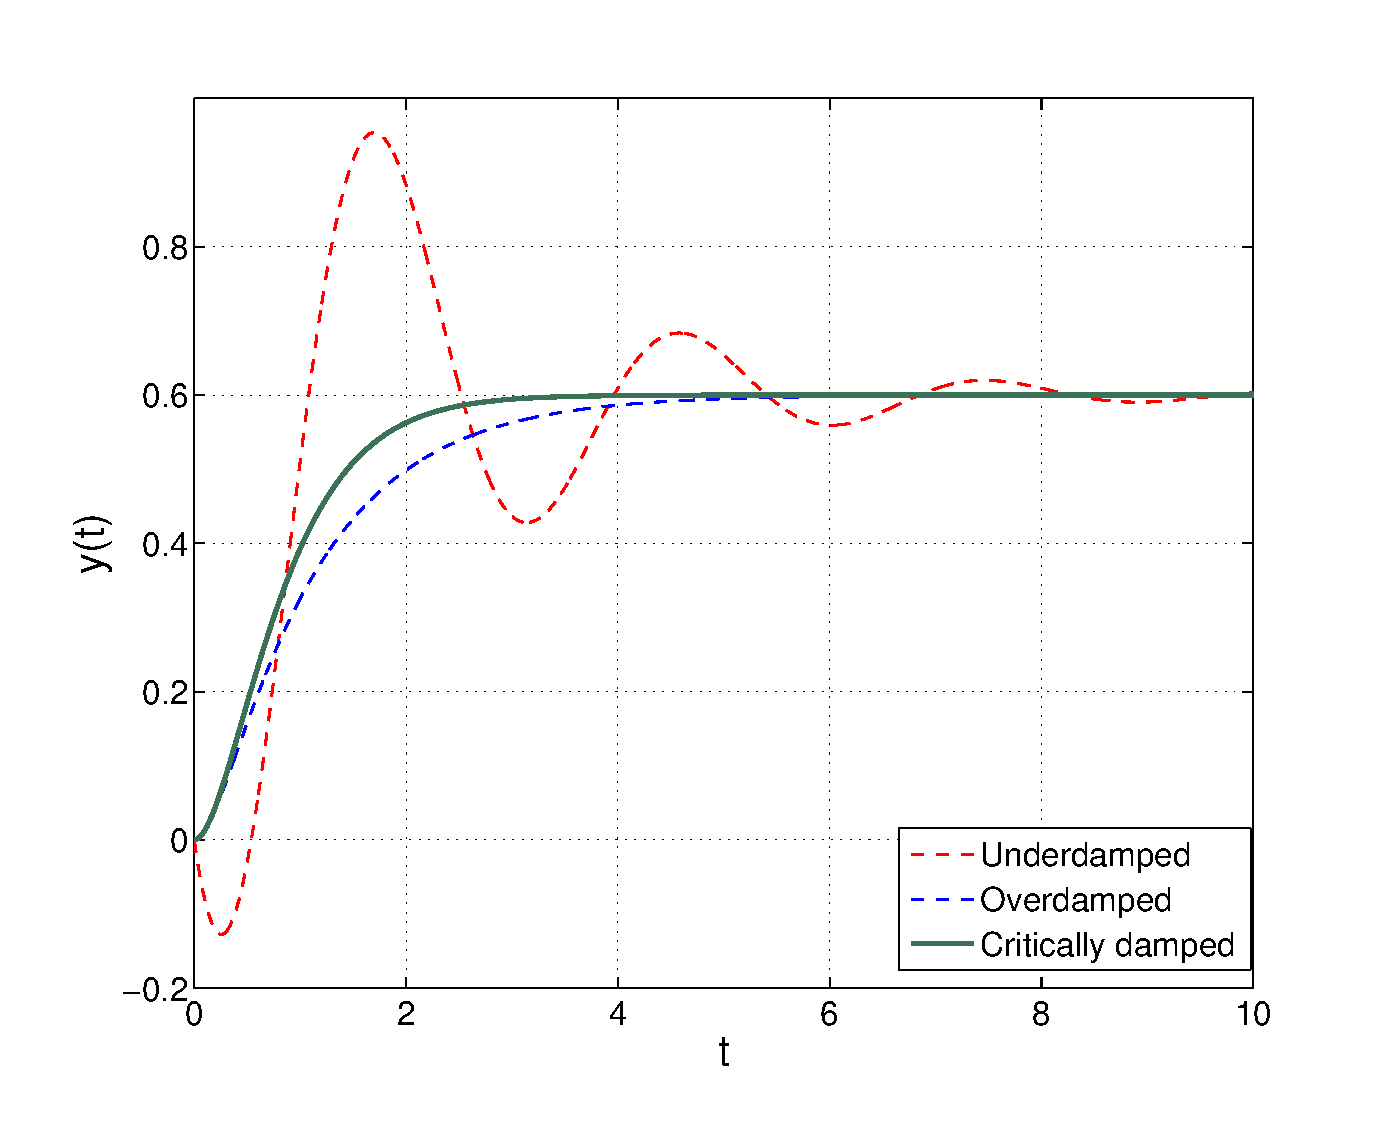
\includegraphics[scale=0.4]{Figures/critically_damped.eps}
%\end{figure}
%
%The response of this system to the unit step is said to be \emph{critically damped}.
%
%}
%
\end{document}
